% Standalone TikZ figure: build with `pdflatex paper/figures/system_diagram.tex`
% to produce system_diagram.pdf, then \includegraphics it from main.tex.
% Standalone is used so the main paper preamble does not need tikz.
\documentclass[border=4pt]{standalone}
\usepackage{tikz}
\usetikzlibrary{positioning, arrows.meta, shapes.geometric, fit, calc}

\tikzset{
  block/.style    ={draw, rounded corners, align=center,
                    minimum height=8mm, minimum width=22mm,
                    font=\small\sffamily},
  estimator/.style={block, fill=blue!8},
  controller/.style={block, fill=orange!10},
  advisor/.style  ={block, fill=green!10},
  safety/.style   ={block, fill=red!10},
  sensor/.style   ={block, fill=gray!10, minimum width=18mm},
  arrow/.style    ={-Latex, thick}
}

\begin{document}
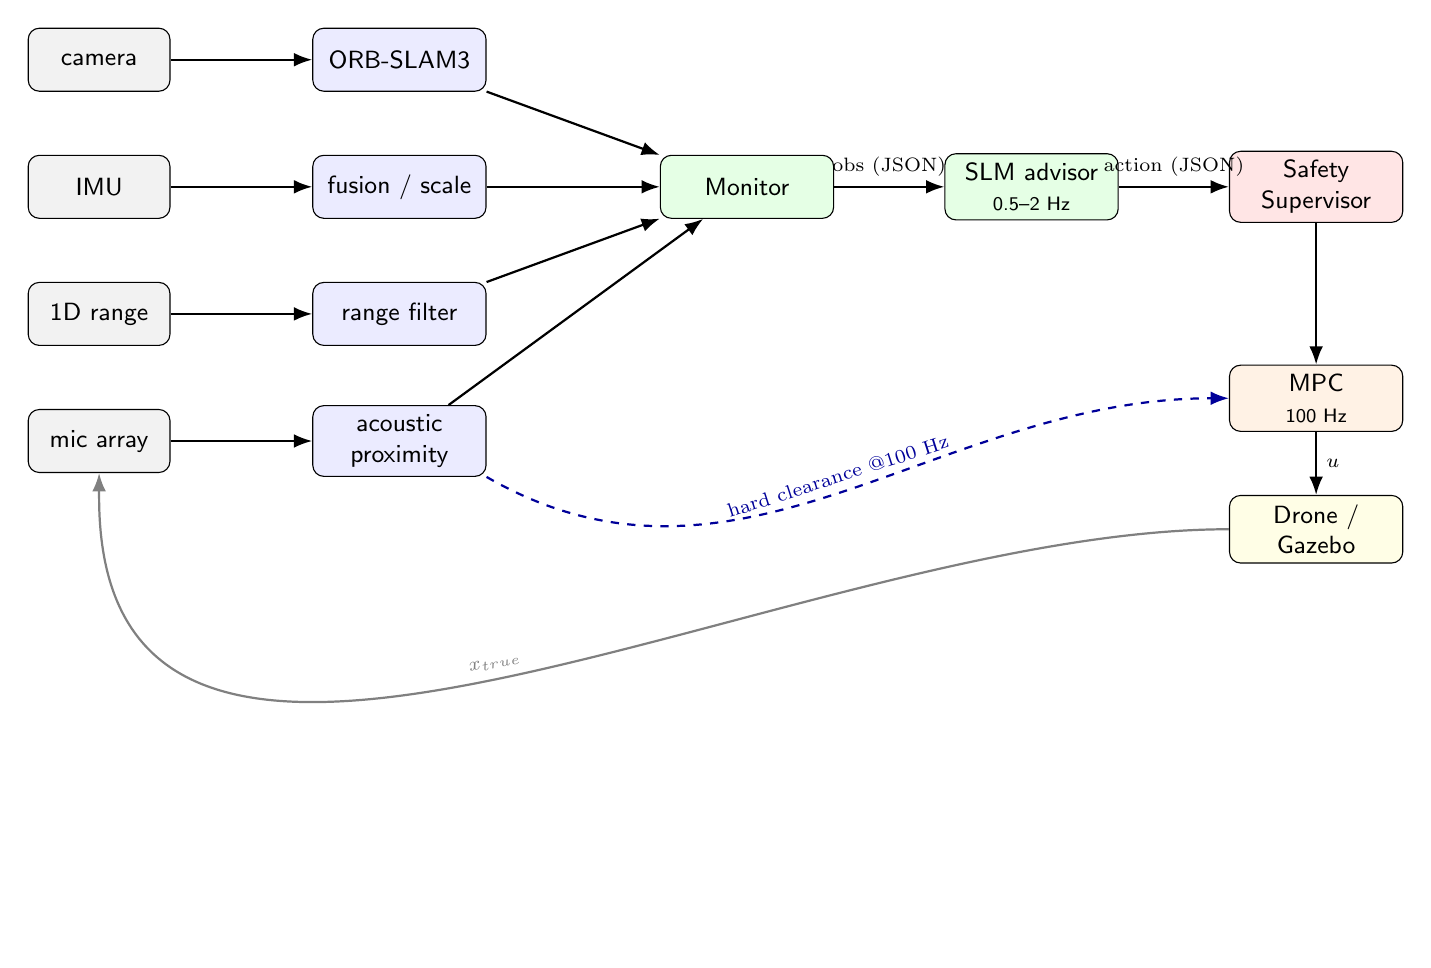
\begin{tikzpicture}[node distance=8mm and 7mm]

  % Sensors
  \node[sensor]                          (cam)   {camera};
  \node[sensor, below=of cam]            (imu)   {IMU};
  \node[sensor, below=of imu]            (rng)   {1D range};
  \node[sensor, below=of rng]            (mic)   {mic array};

  % Estimators
  \node[estimator, right=18mm of cam]    (slam)  {ORB-SLAM3};
  \node[estimator, right=18mm of imu]    (fusion){fusion / scale};
  \node[estimator, right=18mm of rng]    (rngn)  {range filter};
  \node[estimator, right=18mm of mic]    (acn)   {acoustic\\proximity};

  % Monitor + advisor + safety
  \node[advisor, right=22mm of fusion]   (mon)   {Monitor};
  \node[advisor, right=14mm of mon]      (slm)   {SLM advisor\\\scriptsize{0.5--2 Hz}};
  \node[safety, right=14mm of slm]       (saf)   {Safety\\Supervisor};

  % Controller + plant
  \node[controller, below=18mm of saf]   (mpc)   {MPC\\\scriptsize{100 Hz}};
  \node[block, fill=yellow!10, below=of mpc] (drone) {Drone /\\Gazebo};

  % Sensor -> estimator
  \draw[arrow] (cam)  -- (slam);
  \draw[arrow] (imu)  -- (fusion);
  \draw[arrow] (rng)  -- (rngn);
  \draw[arrow] (mic)  -- (acn);

  % Estimator -> Monitor
  \draw[arrow] (slam)   -- (mon);
  \draw[arrow] (fusion) -- (mon);
  \draw[arrow] (rngn)   -- (mon);
  \draw[arrow] (acn)    -- (mon);

  % Monitor -> SLM -> Safety
  \draw[arrow] (mon) -- node[above, font=\scriptsize]{obs (JSON)} (slm);
  \draw[arrow] (slm) -- node[above, font=\scriptsize]{action (JSON)} (saf);

  % Safety -> MPC (waypoint, weights, mode)
  \draw[arrow] (saf) -- (mpc);

  % MPC -> drone
  \draw[arrow] (mpc) -- node[right, font=\scriptsize]{$u$} (drone);

  % Acoustic clearance: hard constraint at controller rate
  \draw[arrow, dashed, blue!60!black]
       (acn.south east) to[out=-30, in=180]
       node[font=\scriptsize, sloped, above]{hard clearance @100 Hz}
       (mpc.west);

  % Drone -> sensors (closing the loop)
  \draw[arrow, gray]
       (drone.west) to[out=180, in=-90]
       node[font=\scriptsize, sloped, above]{$x_{\text{true}}$}
       ($(mic.south)+(0,-3mm)$) -- (mic.south);

\end{tikzpicture}
\end{document}
